\documentclass[11pt]{article}
\usepackage[utf8]{inputenc}
\usepackage[T1]{fontenc}
\usepackage{graphicx}
\usepackage{hyperref}

\author{Student: Sean Wang, szw87 \\ Professor: Mohit Tiwari, Antonio Espinoza \\ Department of Electrical \& Computer Engineering \\ The University of Texas at Austin}
\date{\today}
\title{EE379K Enterprise Network Security Lab 1 Report}
\hypersetup{
 pdfauthor={Student: Sean Wang, szw87 \\ Professor: Mohit Tiwari, Antonio Espinoza \\ Department of Electrical \& Computer Engineering \\ The University of Texas at Austin},
 pdftitle={EE379K Enterprise Network Security Lab 1 Report},
 pdfkeywords={},
 pdfsubject={},
 pdfcreator={},
 pdflang={English}}

\begin{document}

\maketitle
\section*{Part 1:}
\subsection*{Step 1:}
For step 1, the client and server in C were implemented to closely match the Python versions.
For simplicity, the client sends the same hard coded message each time, similar to the Python
client. The C client and server were tested with the Python client and server to ensure
cross-functionality and that the client implementation in both languages worked almost
identically. The only difference between the C client and Python client was the output of the
Python client showing
\begin{center}
  \verb|From Server: b'INPUT LOWERCASE SENTENCE:'|
\end{center}
and the C client showing
\begin{center}
  \verb|From Server: INPUT LOWERCASE SENTENCE:|.
\end{center}
To build the server, compile it with:
\begin{center}
  \verb|gcc -o server server.c|
\end{center}
Similarly for the client, compile it with:
\begin{center}
  \verb|gcc -o client client.c|
\end{center}
To run them, simply execute either:
\begin{center}
  \verb|./server| or \verb|./client|
\end{center}
\subsection*{Step 2:}
For step 2, the DOS attack was implemented using a command line tool called \verb|hping3| using
the options
\begin{center}
  \verb|hping3 --count 15000 --destport 12000|\\
  \verb|--syn --flood --rand-source 127.0.0.2|
\end{center}
These flags specify to stop sending packets to \verb|127.0.0.2:12000| after sending/receiving 15000
SYN packets, using randomized IP addresses to disguise the actual source and prevent the
server's SYN-ACK packets from reaching the actual source. Additionally, the \verb|--flood|
option just says to send packets as fast as possible.\\
As a result, the server receives many requests for establishing a connection, but because the
SYN-ACK sent from the server never reaches the actual sender of the initial SYN packet, the
3-way handshake is never completed and the server is left waiting on a response from what it
sees as many clients. This can be seen in Figure~\ref{fig:handshake}, with some packet details
cut out to ensure legibility.
\begin{figure}[htbp]
  \centering
  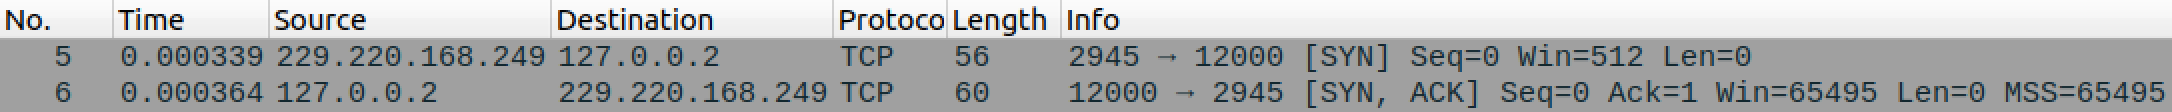
\includegraphics[width=1\linewidth]{./incomplete_handshake.png}
  \caption{\label{fig:handshake}
  An incomplete three-way handshake}
\end{figure}
\\
Since the server is now swamped with connection requests, the real client (at IP \verb|127.0.0.1|)
cannot have its connection request processed by the server and times out, as shown in
Figure~\ref{fig:timeout}, also with some packet details cut out to ensure legibility.
\begin{figure}[htbp]
  \centering
  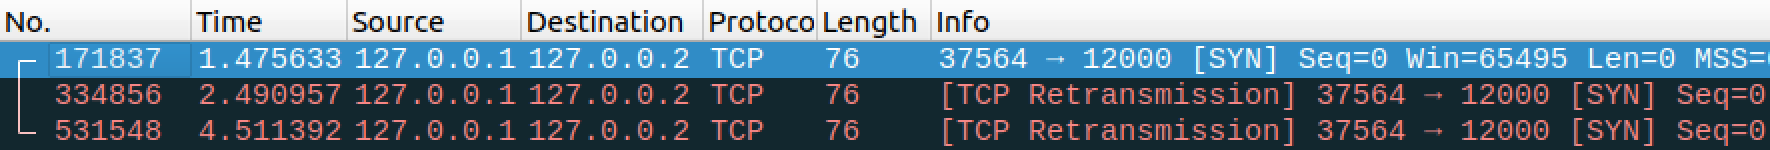
\includegraphics[width=1\linewidth]{./client_timeout.png}
  \caption{\label{fig:timeout}
  Client's sent SYN packet and client timeout}
\end{figure}
\\
The rest of the tcpdump record of the DOS attack is in \verb|output.pcap| and shows the flood
of SYN packets sent to the server at IP \verb|127.0.0.2:12000|.
\section*{Part 2:}

% \label{part1:step-1}
% Nam dui ligula, fringilla a, euismod sodales, sollicitudin vel, wisi. Morbi
% auctor lorem non justo. Nam lacus libero, pretium at, lobortis vitae, ultricies
% et, tellus. Donec aliquet, tortor sed accumsan bibendum, erat ligula aliquet
% magna, vitae ornare odio metus a mi. Morbi ac orci et nisl hendrerit mollis.
% Suspendisse ut massa. Cras nec ante. Pellentesque a nulla. Cum sociis natoque
% penatibus et magnis dis parturient montes, nascetur ridiculus mus. Aliquam
% tincidunt urna. Nulla ullamcorper vestibulum turpis. Pellentesque cursus luctus
% mauris.

\end{document}
